\chapter{Perpetuus, uma \emph{Gem} para construir MVP's}
\label{cap:gem}

% - - - - - - - - - - - - - - - - - - - - - - - - - - - - - - - - - - -
\section{O conceito de Gem}

Uma Gem pode ser definida como um pacote ou uma aplica\c{c}\~ao escrito em linguagem Ruby \cite{berube2007practical}. Essas bibliotecas podem ser divulgadas e instaladas em diversos computadores que tenham suporte \`a linguagem Ruby instalado.

Gems s\~ao escritas em sua maioria com o intuito de automatizar tarefas repetitivas e fornecer solu\c{c}\~oes a problemas comuns a muitos desenvolvedores.

\section{Descri\c{c}\~ao da Perpetuus Gem}

A \emph{gem} Perpetuus foi desenvolvida para garantir que desenvolvedores \emph{web} possam construir MVP's baseados no \emph{framework} Ruby on Rails, isso permite que \emph{startups} testem suas hip\'oteses de mercado utilizando um ambiente que acelere a produ\c{c}\~ao de um produto na \emph{internet}.

Perpetuus oferece um \emph{template} de aplica\c{c}\~ao Ruby on Rails integrado com o \emph{framework} RSpec para atender \`as boas pr\'aticas de programa\c{c}\~ao orientada \`a escrita de testes, dentro do pacote o desenvolvedor tamb\'em conta com um script para gera\c{c}\~ao autom\'atica do reposit\'orio de versionamento de c\'odigo utilizando o GitHub, 

\section{Requisitos de Sistema}

Para utilizar o plugin desenvolvido os seguintes requisitos de sistema precisam ser preenchidos:

\begin{itemize}
\item Sistema operacional Unix
\item Ruby 1.9 ou superior
\item Rubygems 2.0 ou superior
\item Cliente Git
\item Heroku Toolbelt
\item Bundler 1.3 ou superior
\end{itemize} 

\section{Tecnologias Empregadas}

\subsection{Ruby}

Ruby \'e uma linguagem de programa\c{c}\~ao de script interpretada, criada em 1994 por Yukihiro Matsumoto, com grande inspira\c{c}\~ao nas linguagens Python e Perl. A linguagem possui a caracter\'istica de ser totalmente orientada a objeto, c\'odigo aberto e com tipagem din\^amica e forte.

Existe uma filosofia por tr\'as do Ruby, a linguagem foi desenvolvida objetivando as pessoas, buscando uma maior produtividade e fornecendo uma sintaxe muito limpa e elegante. Ruby foi projetada com o princ\'ipio da menor surpresa, tentando diminuir a frustra\c{c}\~ao durante a programa\c{c}\~ao. Seu criador tinha o objetivo de fazer uma linguagem que proporcionasse divers\~ao ao programador, diminuindo as dificuldades no desenvolvimento \cite{flanagan2008ruby}.

\subsection{Ruby on Rails}

Antes de descrever sobre o Ruby on Rails ser\'a necess\'ario entender o conceito de framework. Segundo \cite{hartl2012ruby}, framework \'e uma solu\c{c}\~ao para um conjunto de problemas em comum com o uso de classes e interfaces que disponibilizam objetos com funcionalidades comuns a v\'arias aplica\c{c}\~oes. A utiliza\c{c}\~ao de framework pode trazer benef\'icios em rela\c{c}\~ao \`a agilidade de desenvolvimento, podendo reduzir seus custos.

Com o Ruby on Rails pode--se desenvolver sistemas para a web utilizando a orienta\c{c}\~ao a objeto e com a estrutura MVC (Modelo, Visualiza\c{c}\~ao, Controle) para constru\c{c}\~ao em camadas. O framework possui alguns princ\'ipios baseados no desenvolvimento \'agil, com o conceito do Do not Repeat Yourself (DRY, N\~ao se repita), ou seja, n\~ao repetir c\'odigo, e Convention over Configuration (CoC, Conven\c{c}\~ao sobre Configura\c{c}\~ao) \cite{akita2006repensando}.

\subsection{RSpec}

RSpec \'e um \emph{framework} de testes escrito em Ruby, permitindo que se descrevam aplica\c{c}\~oes em linguagem de dom\'inio espec\'ifico em ingl\^es domain--specific language (DSL) \cite{chelimsky2010rspec}

Como a maioria dos projetos falha em manter uma documenta\c{c}\~ao atualizada, utilizar o RSpec pode ser uma excelente maneira de se documentar um projeto, pois o resultado dos exemplos executados, quando bem escritos, formam uma especificac\c{c}\~ao do projeto.

\subsection{GitHub}

O GitHub \'e um servi\c{c}o de hospedagem para projetos de desenvolvimento de \emph{software} que usam o sistema de controle de vers\~ao Git. GitHub oferece planos pagos para reposit\'orios privados e contas livres para projetos de c\'odigo aberto (open--source). Em maio de 2011, tornou--se o local mais popular para hospedagem de projetos de c\'odigo--fonte aberto \cite{loeliger2012version}

\subsection{Heroku}

Heroku \'e uma plataforma de hospedagem de servi\c{c}os na nuvem que suporta linguagens de programa\c{c}\~ao como Ruby, Java, PHP e frameworks como Ruby on Rails \cite{kemp2013professional}.

O diferencial do Heroku est\'a na automa\c{c}\~ao da configura\c{c}\~ao necess\'aria \`a cria\c{c}\~ao de um ambiente para colocar uma aplica\c{c}\~ao em funcionamento, assim programadores podem focar seus esfor\c{c}os no desenvolvimento do \emph{software}, ficando a cargo do Heroku juntar os m\'odulos desenvolvidos, resolver quest\~oes de depend\^encia e tornar o que antes era c\'odigo em uma aplica\c{c}\~ao dispon\'ivel aos clientes.

\subsection{Travis}

Travis \'e uma plataforma de servi\c{c}o respons\'avel por automatizar a montagem do c\'odigo fonte que \'e versionado em um reposit\'orio remoto como o GitHub, mais detalhes do servi\c{c}o podem ser encontrados em https://travis-ci.org/

\section{Instala\c{c}\~ao}

Para instalar a gem Perpetuus \'e preciso apenas executar o comando "gem install perpetuus" no terminal de comandos do Sistema Operacional, a instala\c{c}\~ao \'e autom\'atica e n\~ao requer nenhuma intera\c{c}\~ao do usu\'ario durante o processo.

\section{Funcionamento da Gem}

\subsection{O comando \emph{perpetuus setup}}

Para iniciar a constru\c{c}\~ao de um novo projeto, o desenvolvedor utiliza o comando "perpetuus setup", assim \'e poss\'ivel definir a estrutura inicial do MVP que ser\'a constru\'ido seguindo os passos demonstrados nas figuras \ref{fig:fig6}, \ref{fig:fig7}, \ref{fig:fig8}, \ref{fig:fig9}, \ref{fig:fig10}:

Na figura \ref{fig:fig6} \'e pedido ao desenvolvedor que escolha um nome para o seu projeto, pois um novo diret\'orio ser\'a criado com esse nome para guardar os arquivos contidos na estrutura inicial do projeto.

\begin{figure}[h]
  \centering
  \caption{Tela inicial do \emph{plugin} para o usu\'ario inserir o nome do projeto}
  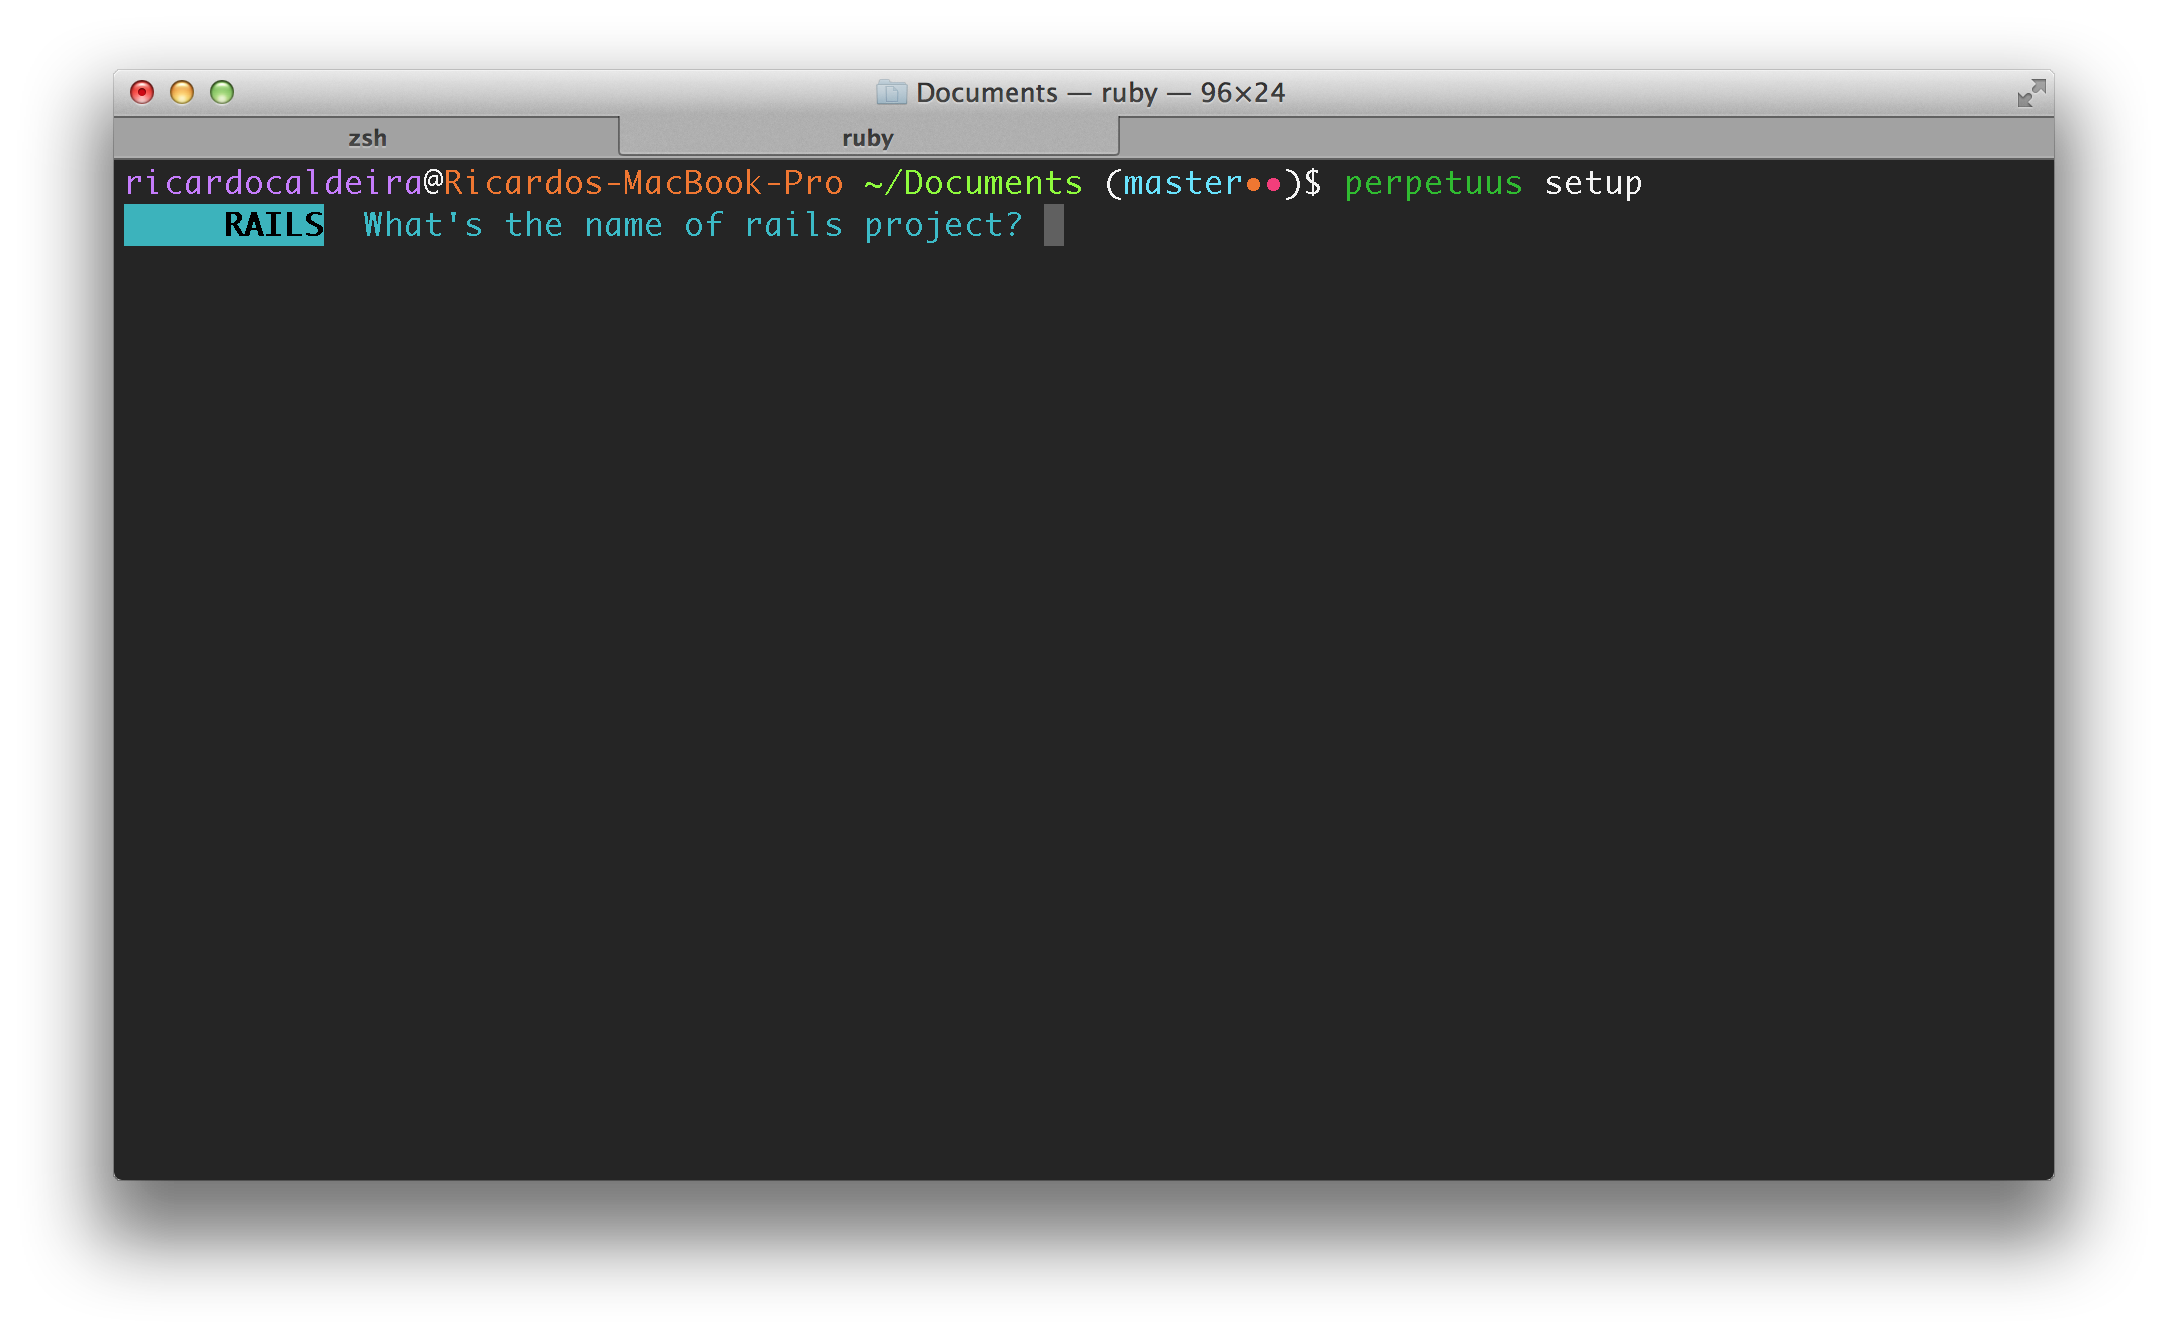
\includegraphics[width=0.5\textwidth]{./fig/setup1}
  \label{fig:fig6}
\end{figure}

A figura \ref{fig:fig7} ilustra a etapa onde \'e perguntado ao desenvolvedor qual banco de dados ele quer utilizar para construir seu MVP.

\begin{figure}[h]
  \centering
  \caption{Tela inicial de defini\c{c}\~ao do banco de dados a ser utilizado.}
  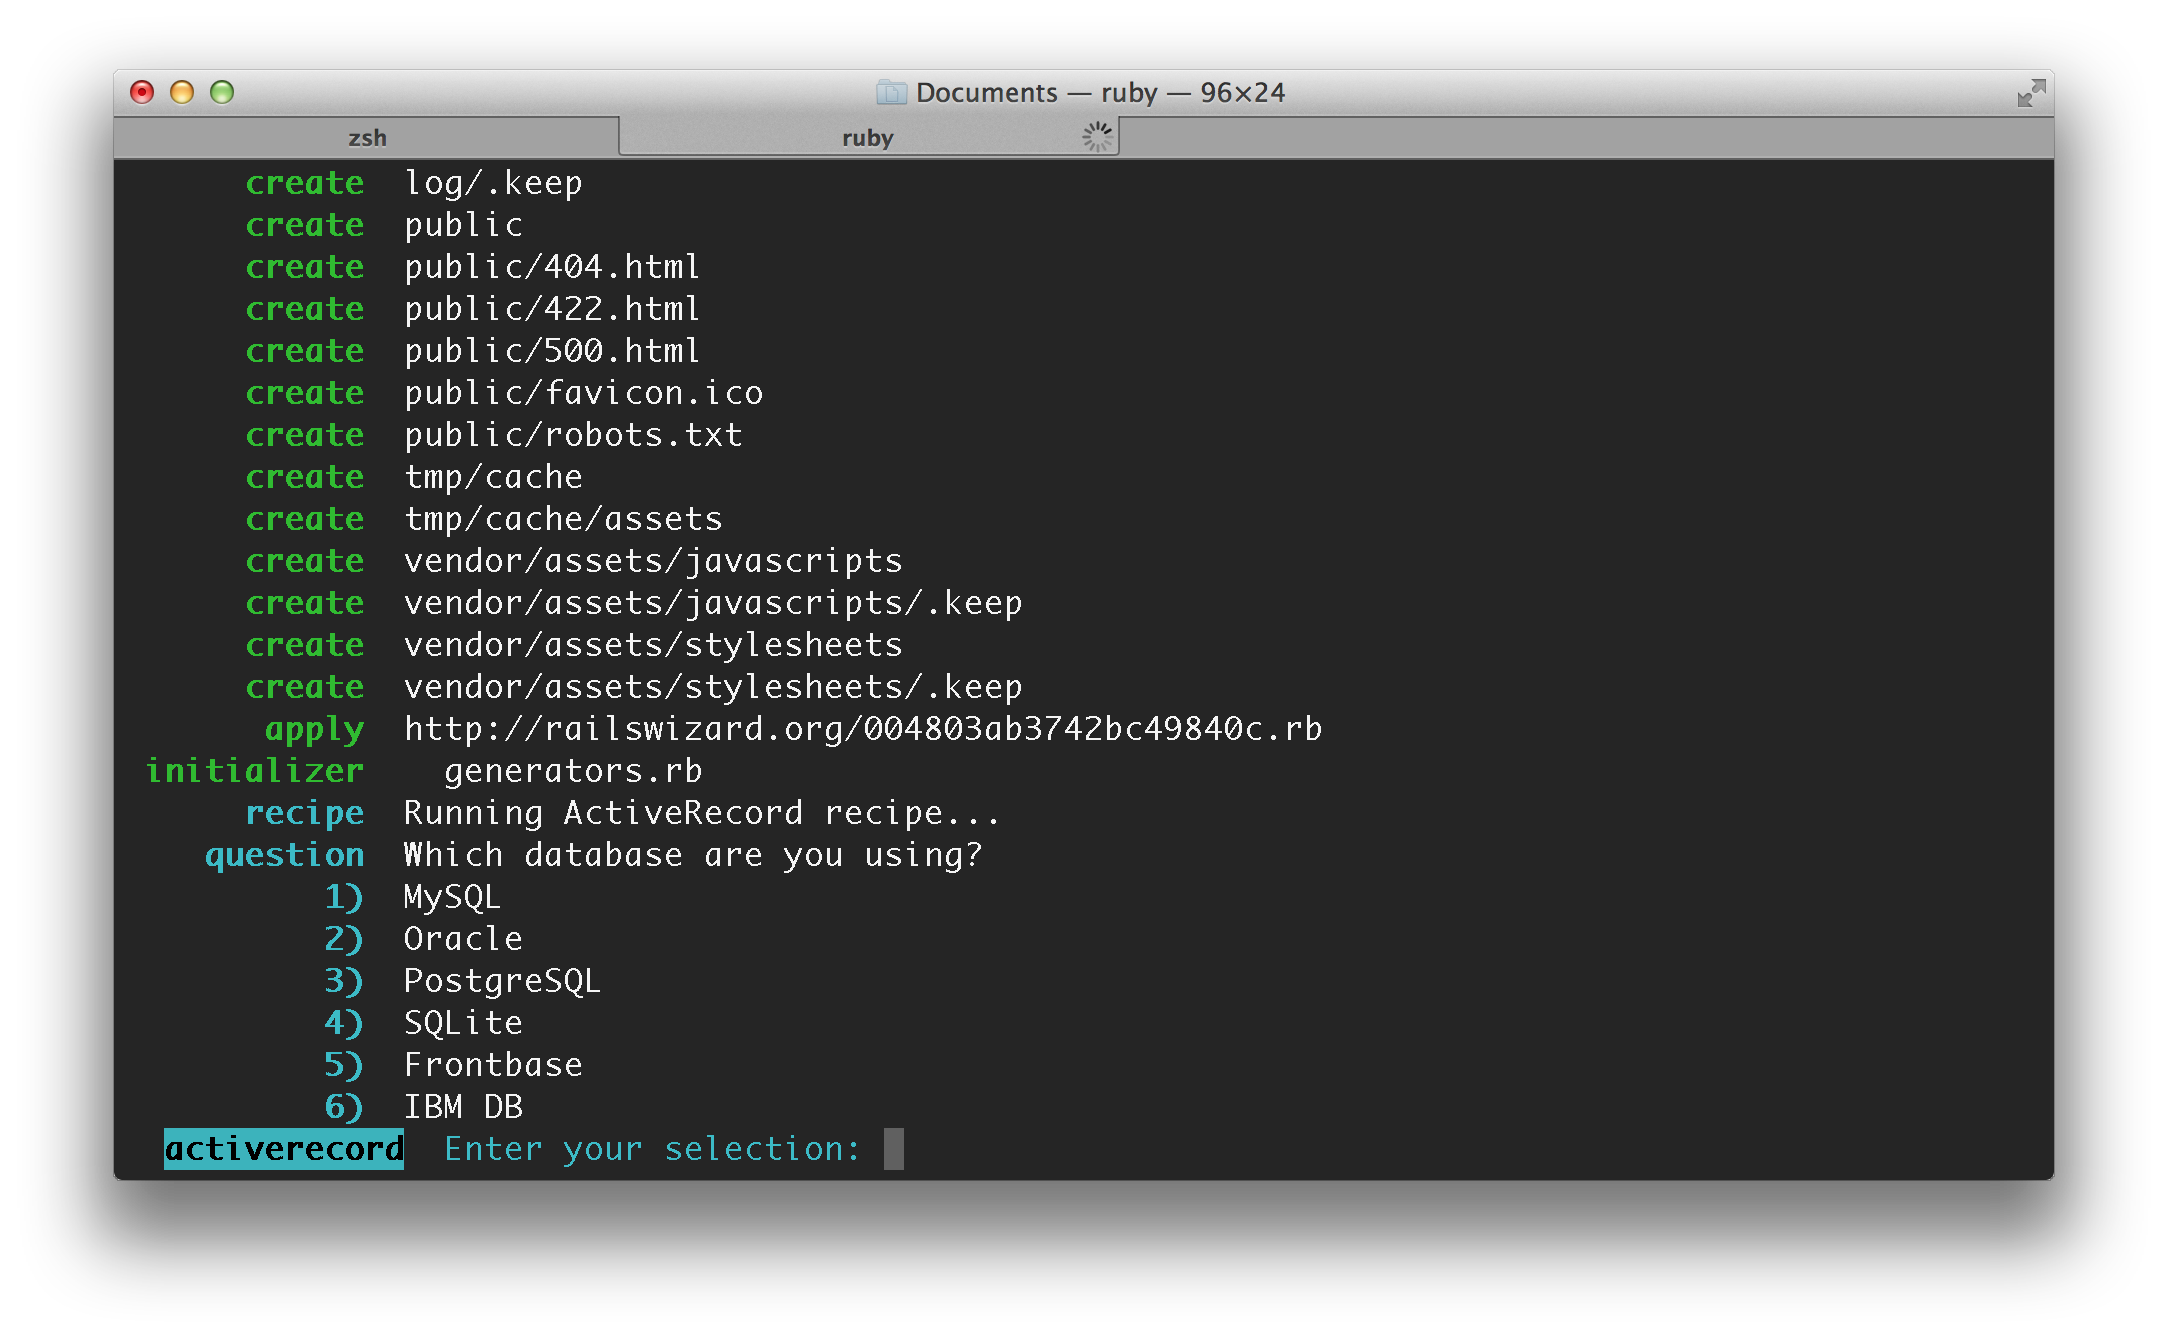
\includegraphics[width=0.5\textwidth]{./fig/setup2}
  \label{fig:fig7}
\end{figure}

Na figura \ref{fig:fig8} o usu\'ario pode deixar a cargo da ferramenta a escolha do nome para a aplica\c{c}\~ao a ser hospedada no Heroku.

\begin{figure}[h]
  \centering
  \caption{Tela para defini\c{c}\~ao do nome do aplicativo.}
  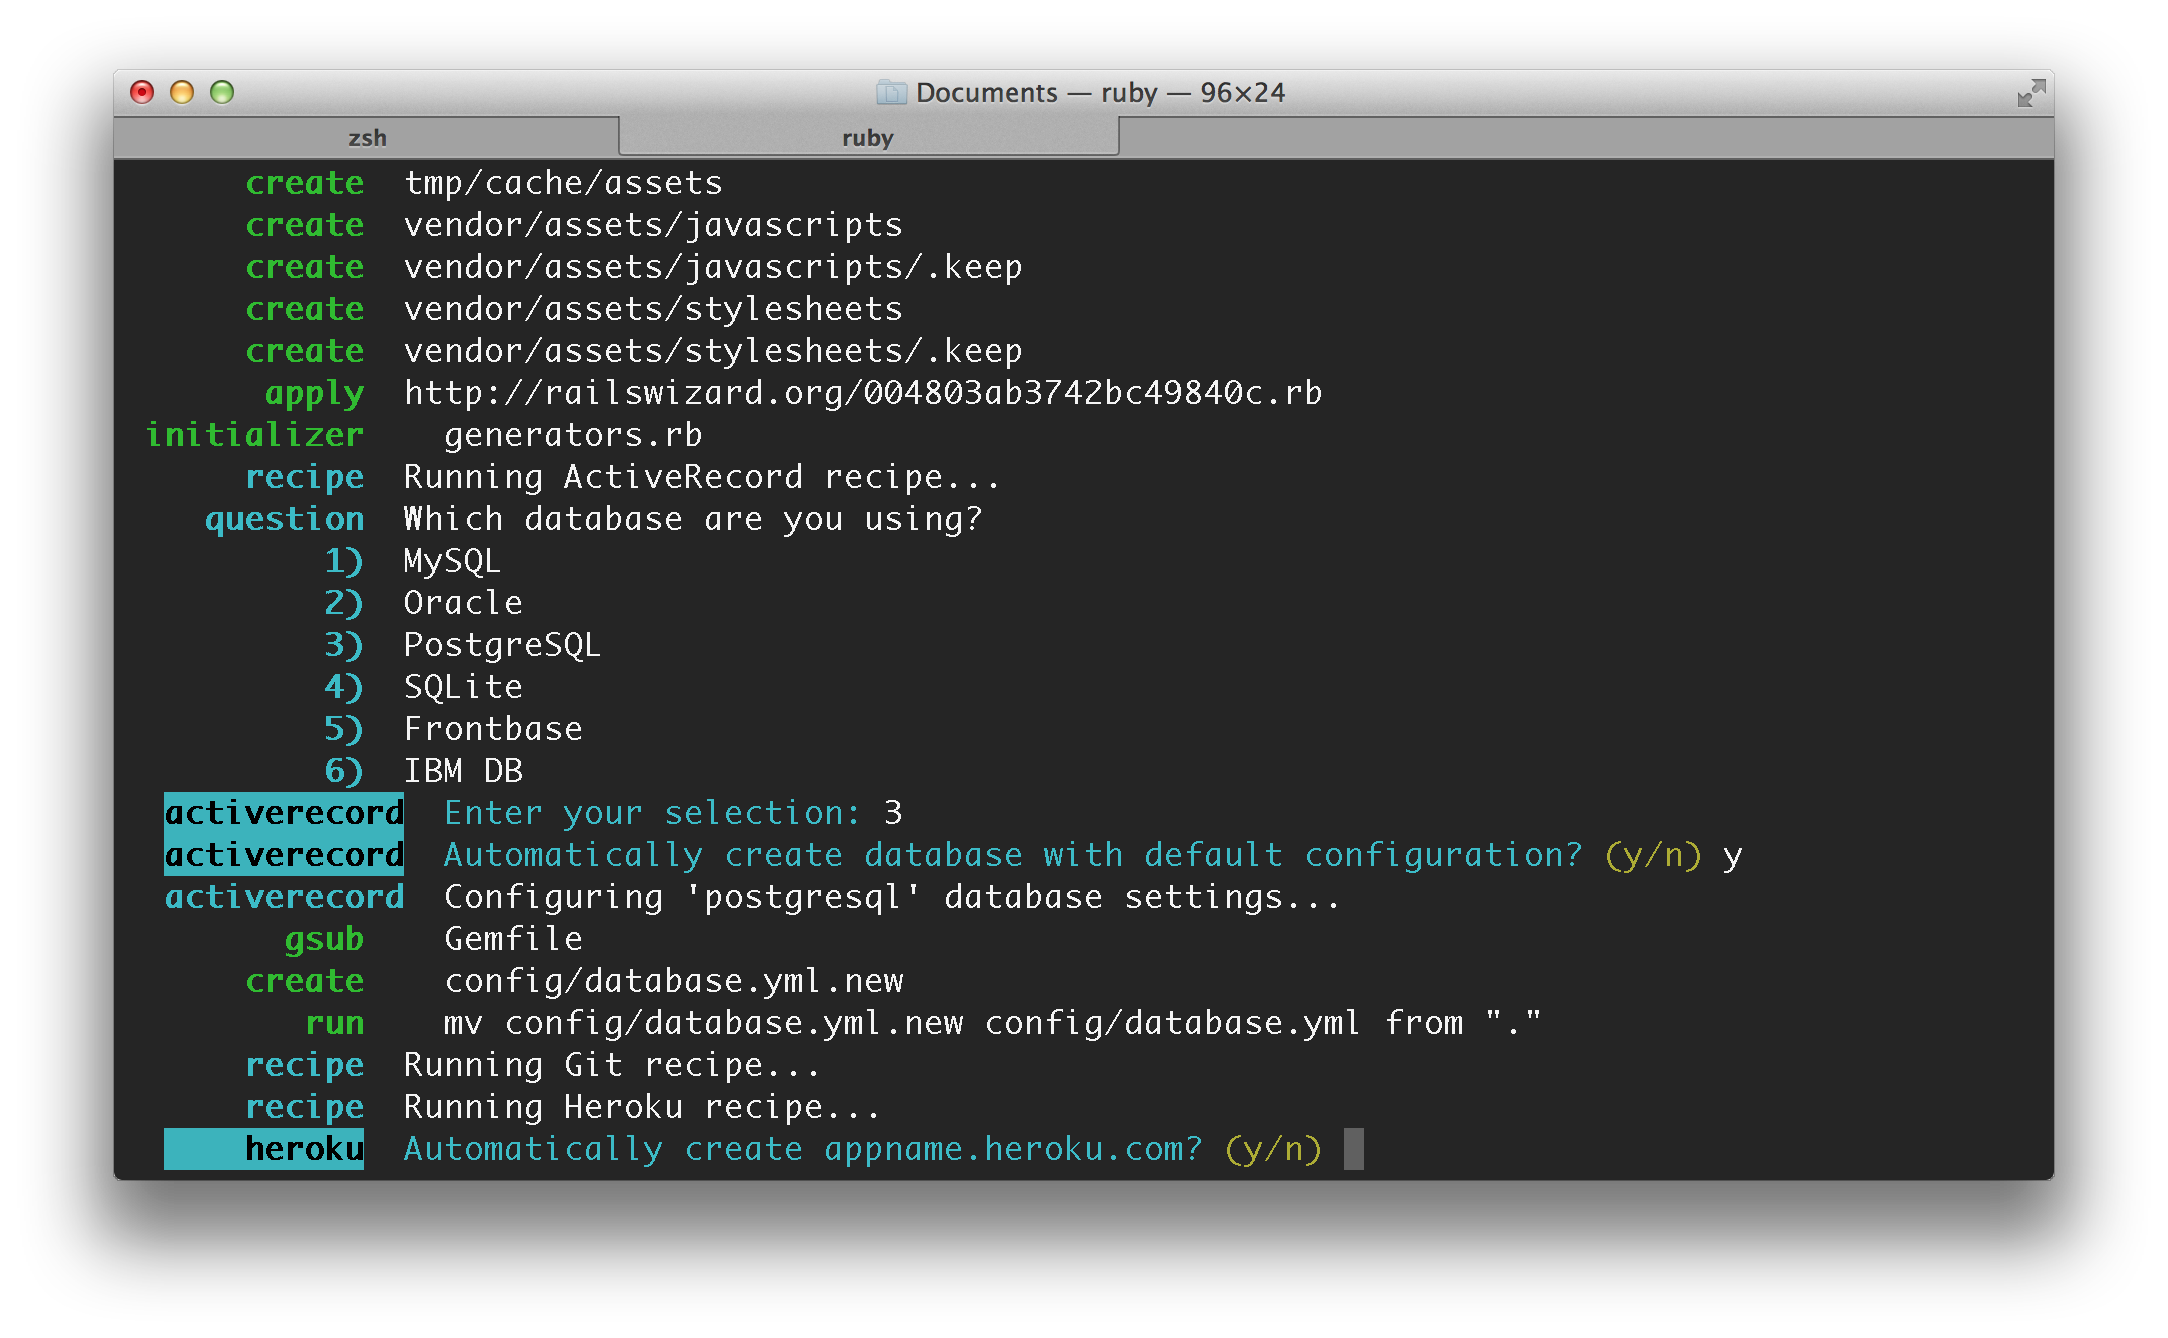
\includegraphics[width=0.5\textwidth]{./fig/setup3}
  \label{fig:fig8}
\end{figure}

\pagebreak

A figura \ref{fig:fig9} mostra o sistema pedindo ao desenvolvedor que defina outro nome para o aplicativo.

\begin{figure}[h]
  \centering
  \caption{Tela para redefini\c{c}\~ao do nome do aplicativo.}
  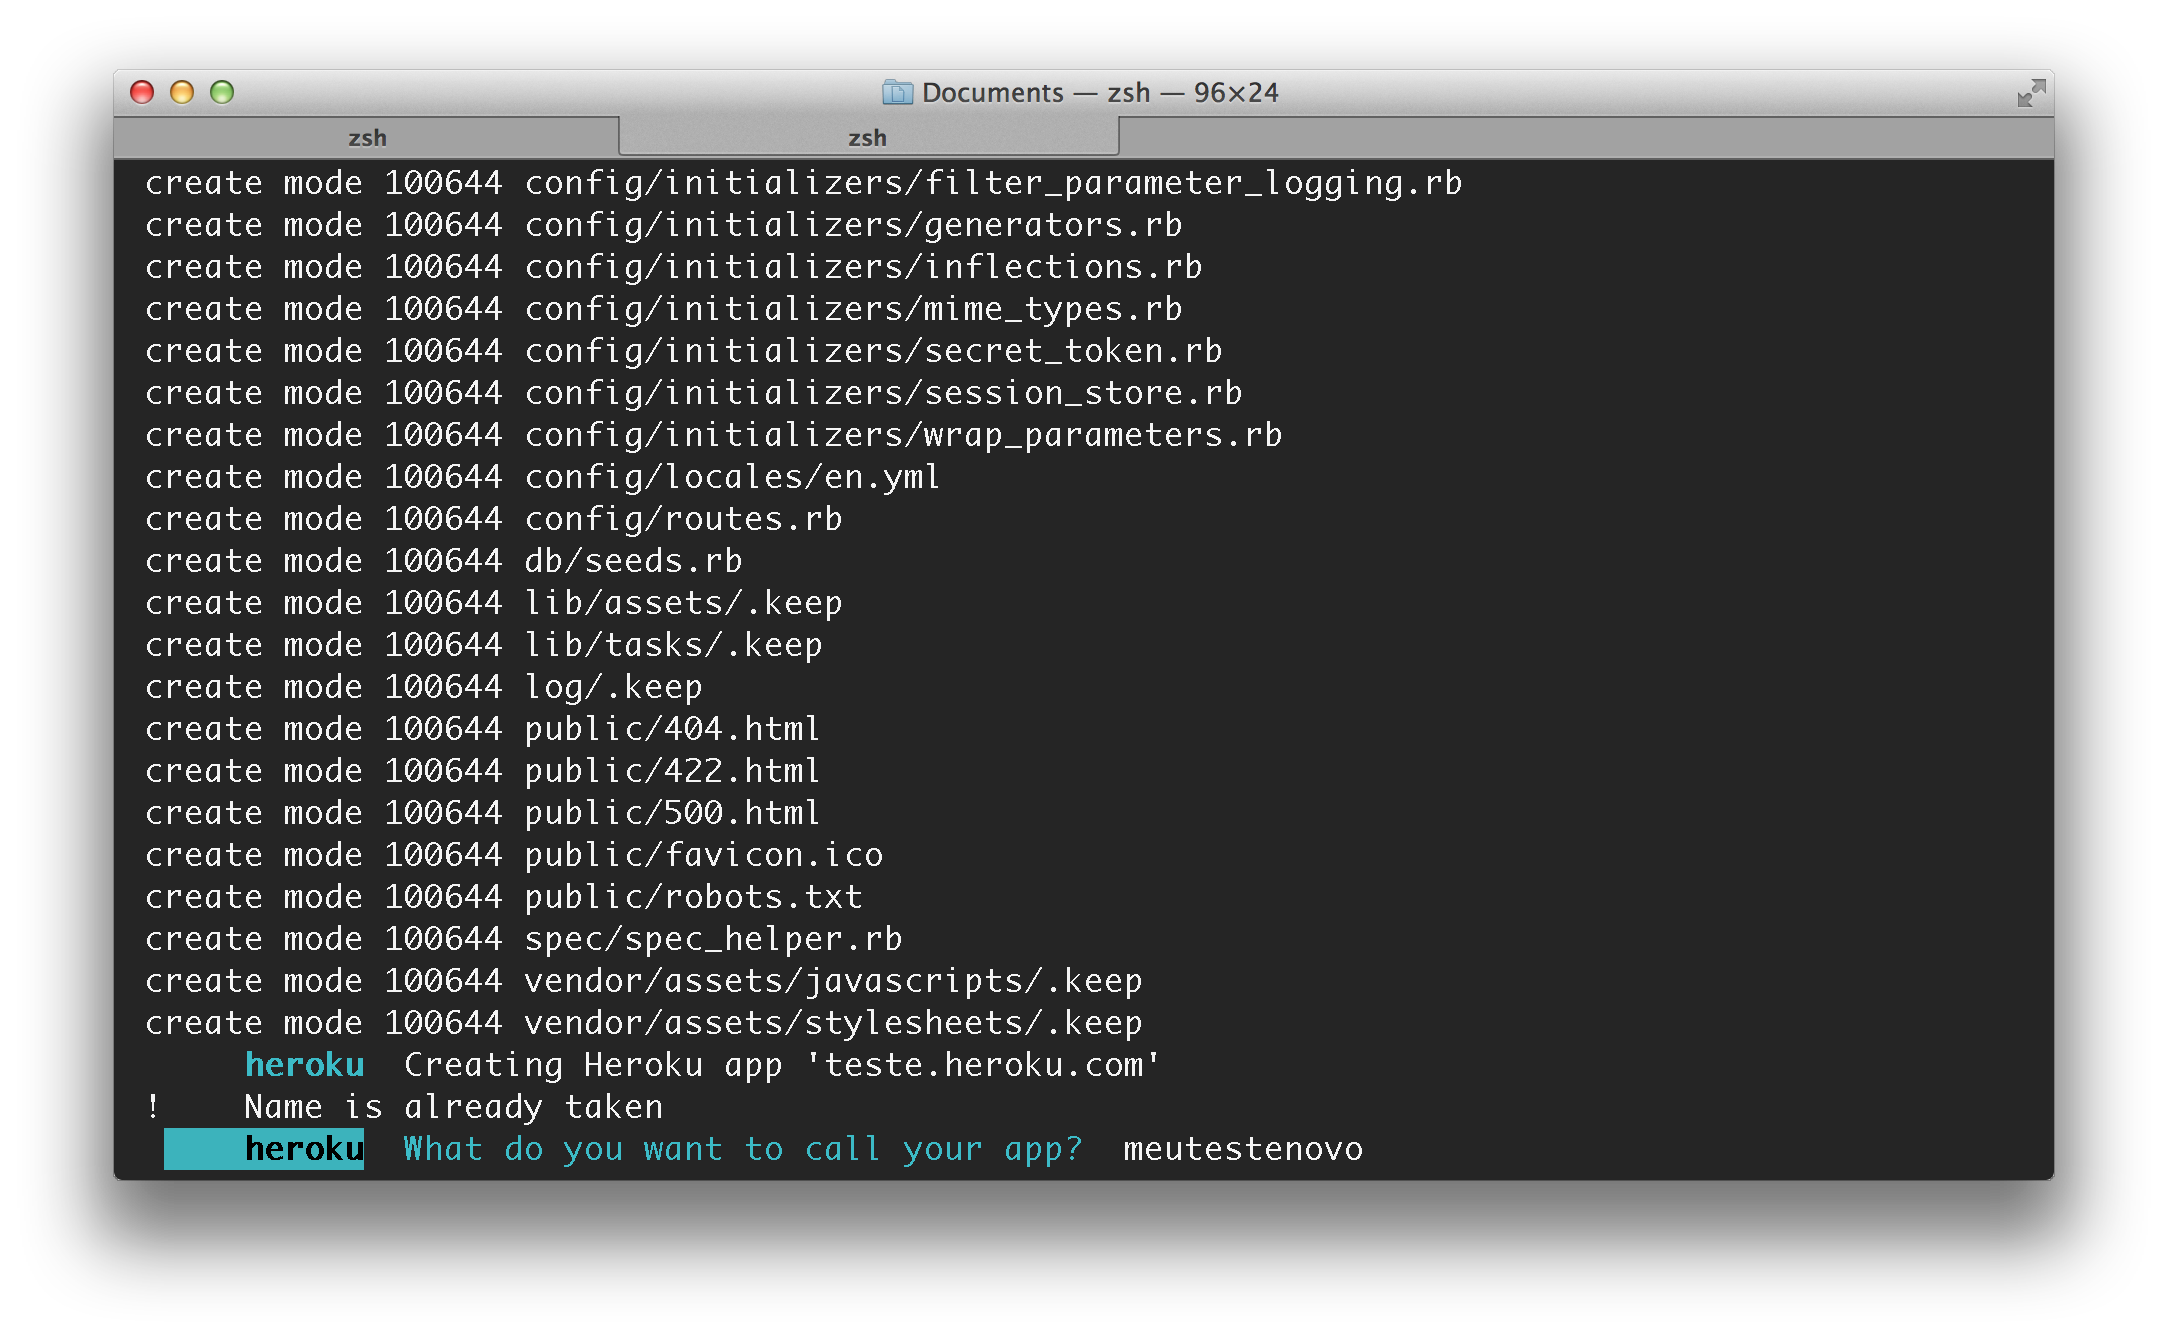
\includegraphics[width=0.5\textwidth]{./fig/setup4}
  \label{fig:fig9}
\end{figure}

A figura \ref{fig:fig10} ilustra a primeira vers\~ao hospedada no servidor de aplica\c{c}\~ao do Heroku, na \'ultima linha \'e poss\'ivel ver o endere\c{c}o na \emph{Internet} onde o aplicativo est\'a hospedado.

\begin{figure}[h]
  \centering
  \caption{Resposta do servidor de hospedagem Heroku.}
  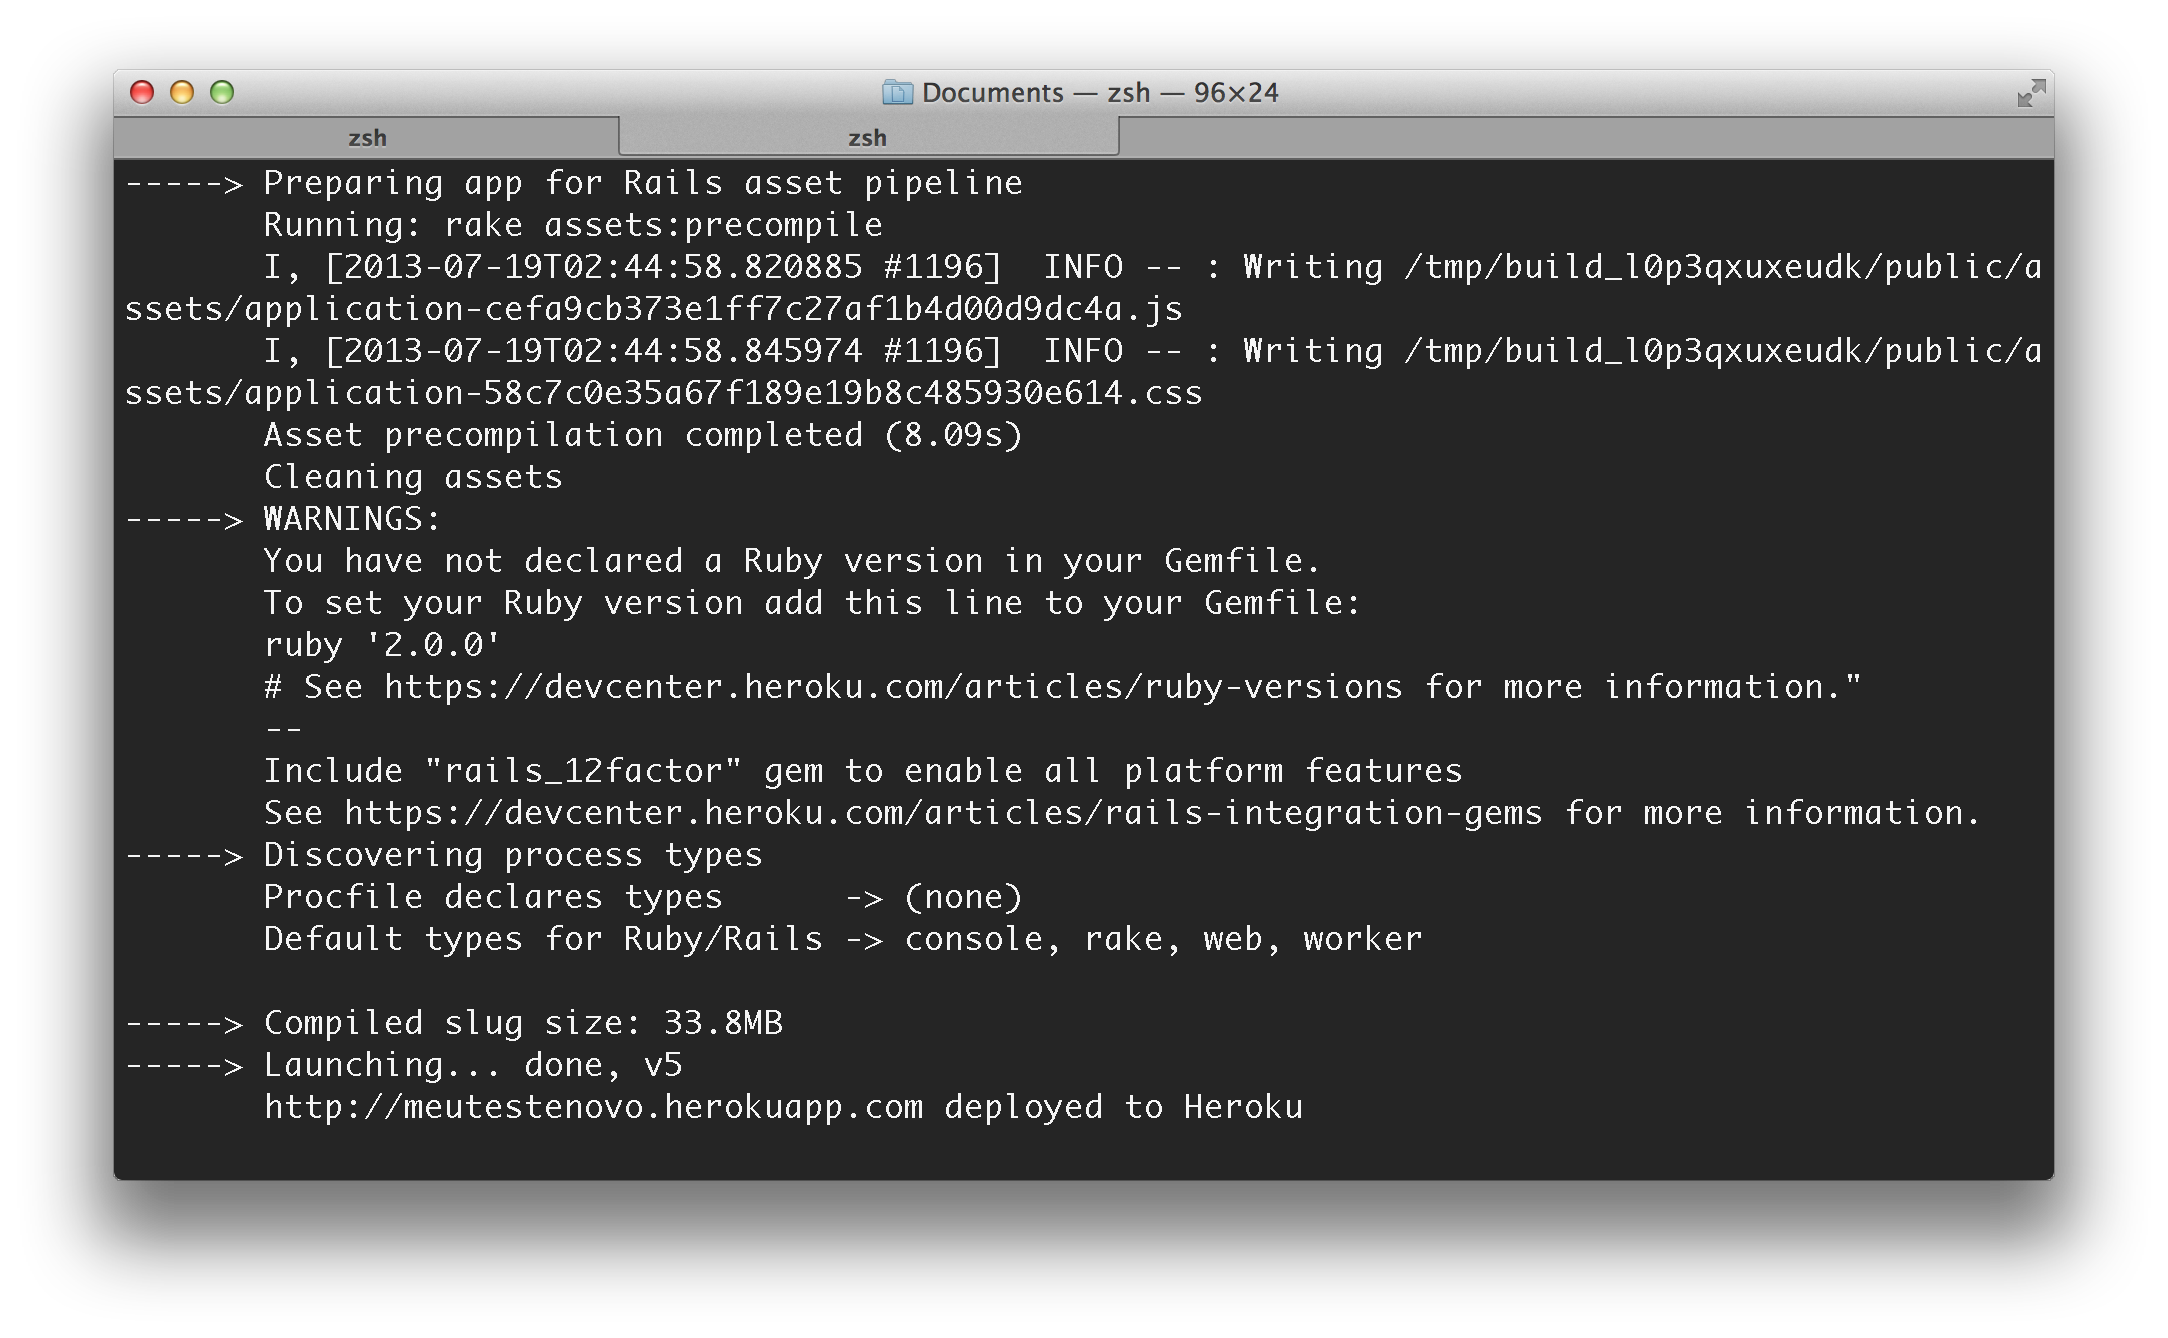
\includegraphics[width=0.5\textwidth]{./fig/setup5}
  \label{fig:fig10}
\end{figure}

\pagebreak
\subsection{O comando \emph{perpetuus deploy}}

Ao executar o comando "perpetuus deploy" em um ambiente pr\'e--configurado pela \emph{gem} o c\'odigo fonte produzido no computador do desenvolvedor \'e primeiramente versionado no reposit\'orio de c\'odigo do GitHub, terminado esse processo \'e a vez do c\'odigo produzido ser montado pelo construtor Travis, nele os testes definidos pelo desenvolvedor (usando o \emph{framework} RSpec) s\~ao executados, caso os testes definidos passem e a aplica\c{c}\~ao consiga ser constru\'ida \'e a vez do c\'odigo ser colocado em produ\c{c}\~ao no servidor de aplica\c{c}\~ao do Heroku, ao final desse processo uma nova vers\~ao de software j\'a est\'a dispon\'ivel aos clientes. 

A figura \ref{fig:fig11} ajuda a ilutrar o caminho do c\'odigo at\'e se tornar um MVP dispon\'ivel aos clientes.

\begin{figure}[h]
  \centering
  \caption{Caminho percorrido pelo c\'odigo fonte at\'e estar dispon\'ivel aos clientes em forma de aplicativo.}
  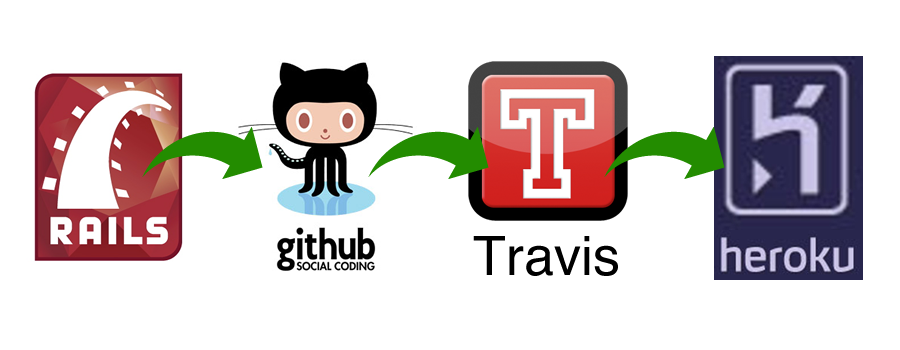
\includegraphics[width=0.6\textwidth]{./fig/cicloDeploy}
  \label{fig:fig11}
\end{figure}

O processo de execu\c{c}\~ao descrito anteriormente exemplifica a constru\c{c}\~ao de \emph{software} baseado em entrega cont\'inua, metodologia ideal para o desenvolvimento de MVP's por permitir r\'apida altera\c{c}\~ao do experimento baseada no \emph{feedback} colhido ao final do ciclo construir--medir--aprender.

\pagebreak

A figura \ref{fig:fig12} mostra um exemplo de tentativa de \emph{deploy} da aplica\c{c}\~ao mal sucedido. Neste caso, um link \'e fornecido ao desenvolvedor com mais detalhes sobre os fatores que impediram o c\'odigo de ser incorporado \`a aplica\c{c}\~ao hospedada no servidor do Heroku.

\begin{figure}[h]
  \centering
  \caption{\emph{Deploy} interrompido por causa de falhas na montagem do aplicativo pelo servi\c{c}o Travis.}
  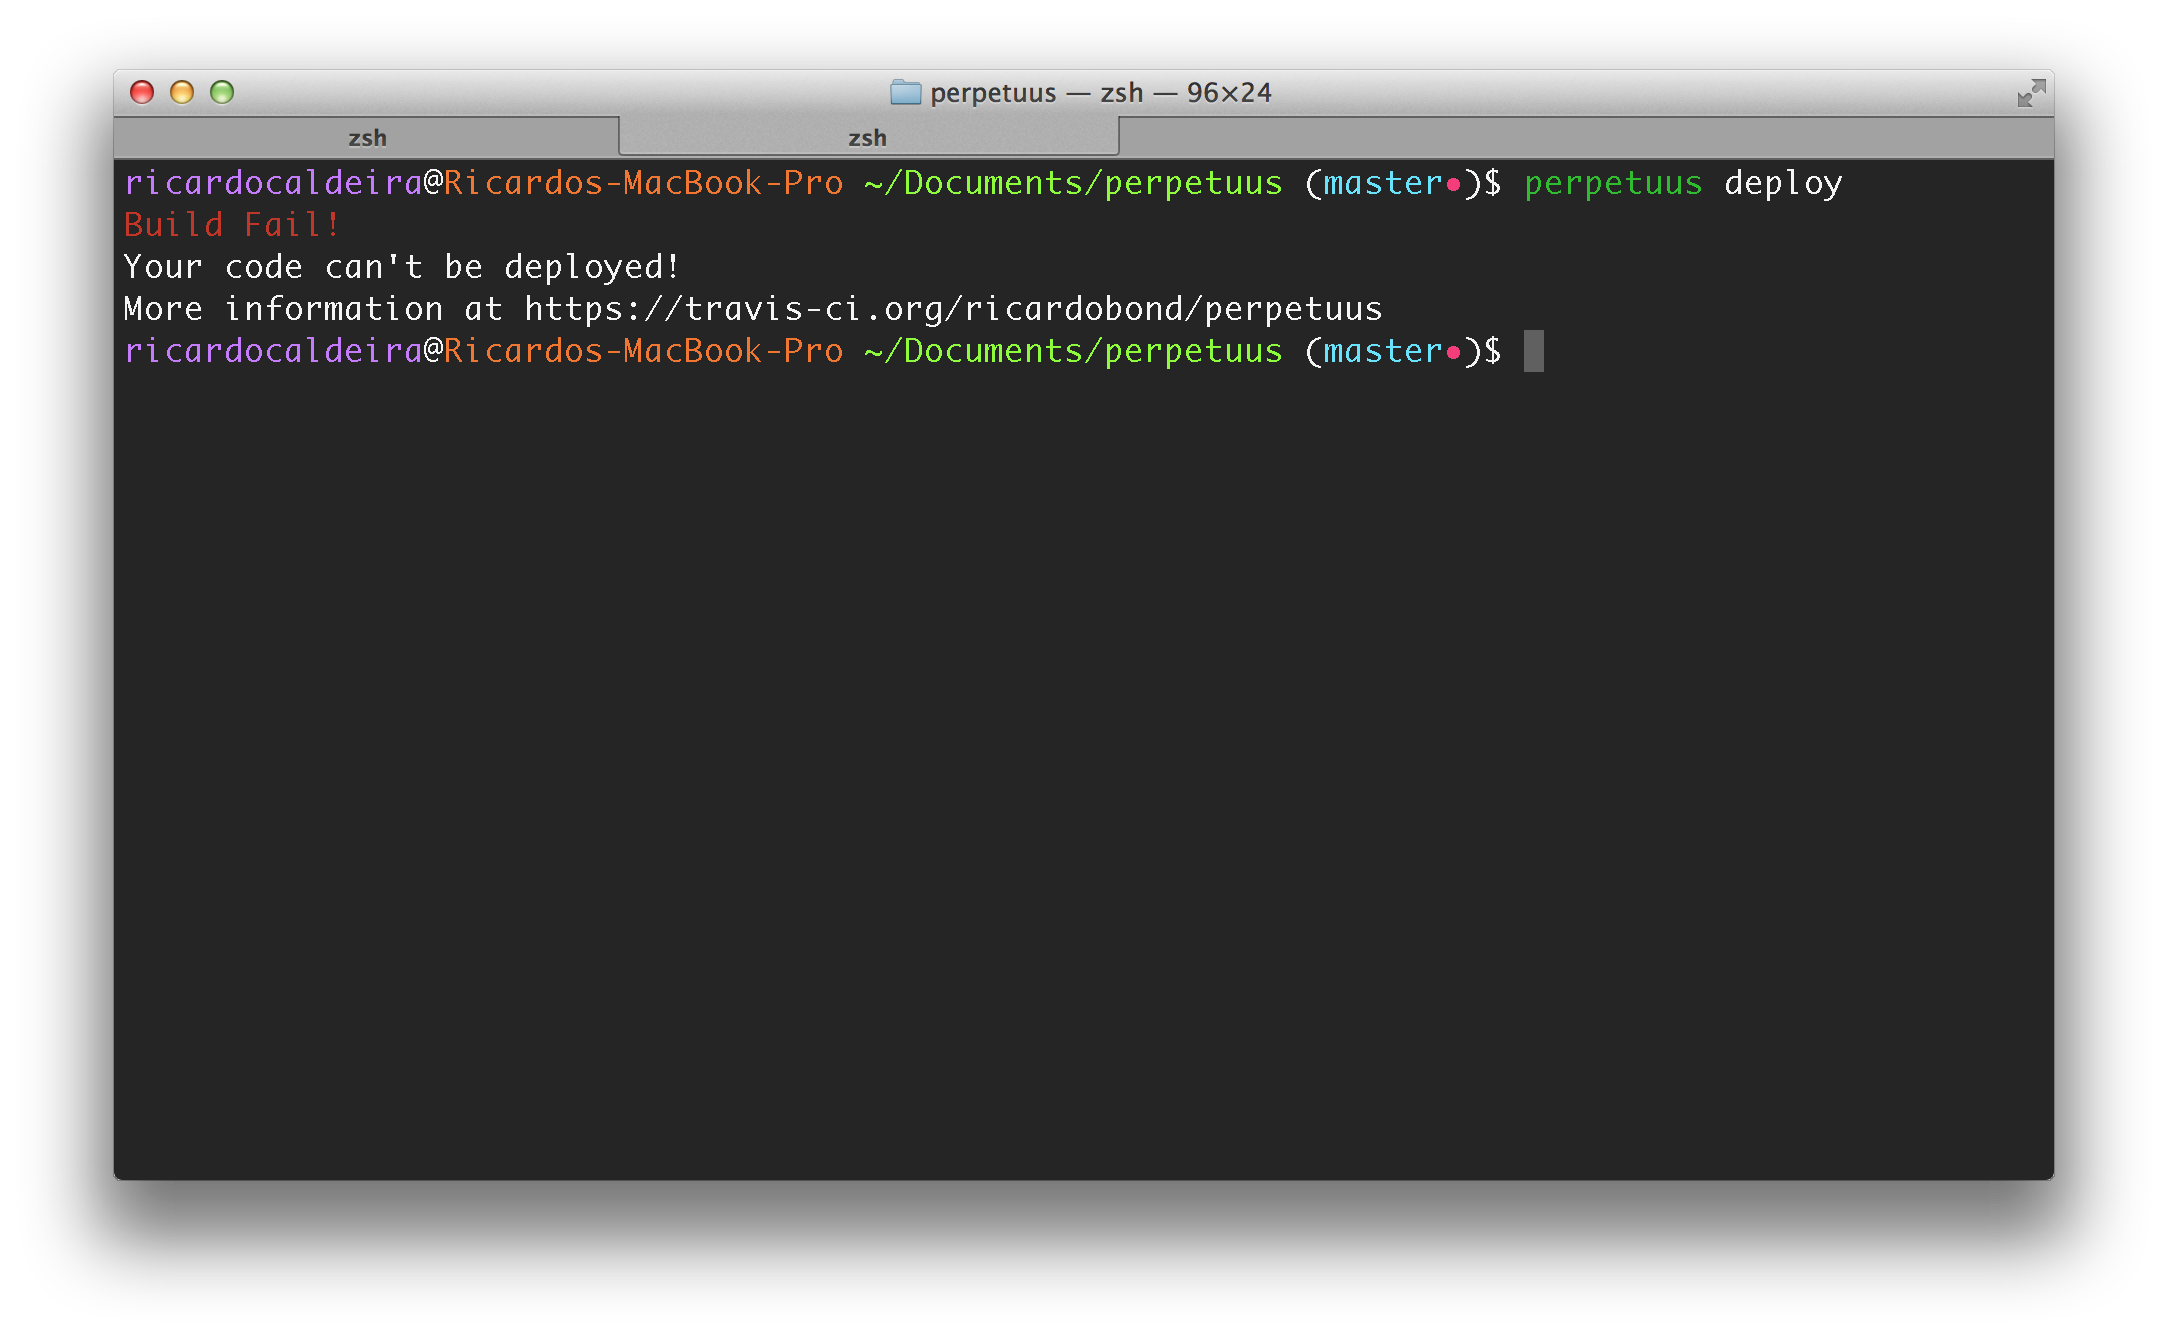
\includegraphics[width=0.5\textwidth]{./fig/deploy1}
  \label{fig:fig12}
\end{figure}

Caso o comando "perpetuus deploy" seja executado com sucesso, a figura \ref{fig:fig13} mostra a o endere\c{c}o onde uma nova vers\~ao do MVP est\'a instalada.

\begin{figure}[h]
  \centering
  \caption{Sa\'ida do console de execu\c{c}\~ao da tarefa de \emph{deploy} do MVP}
  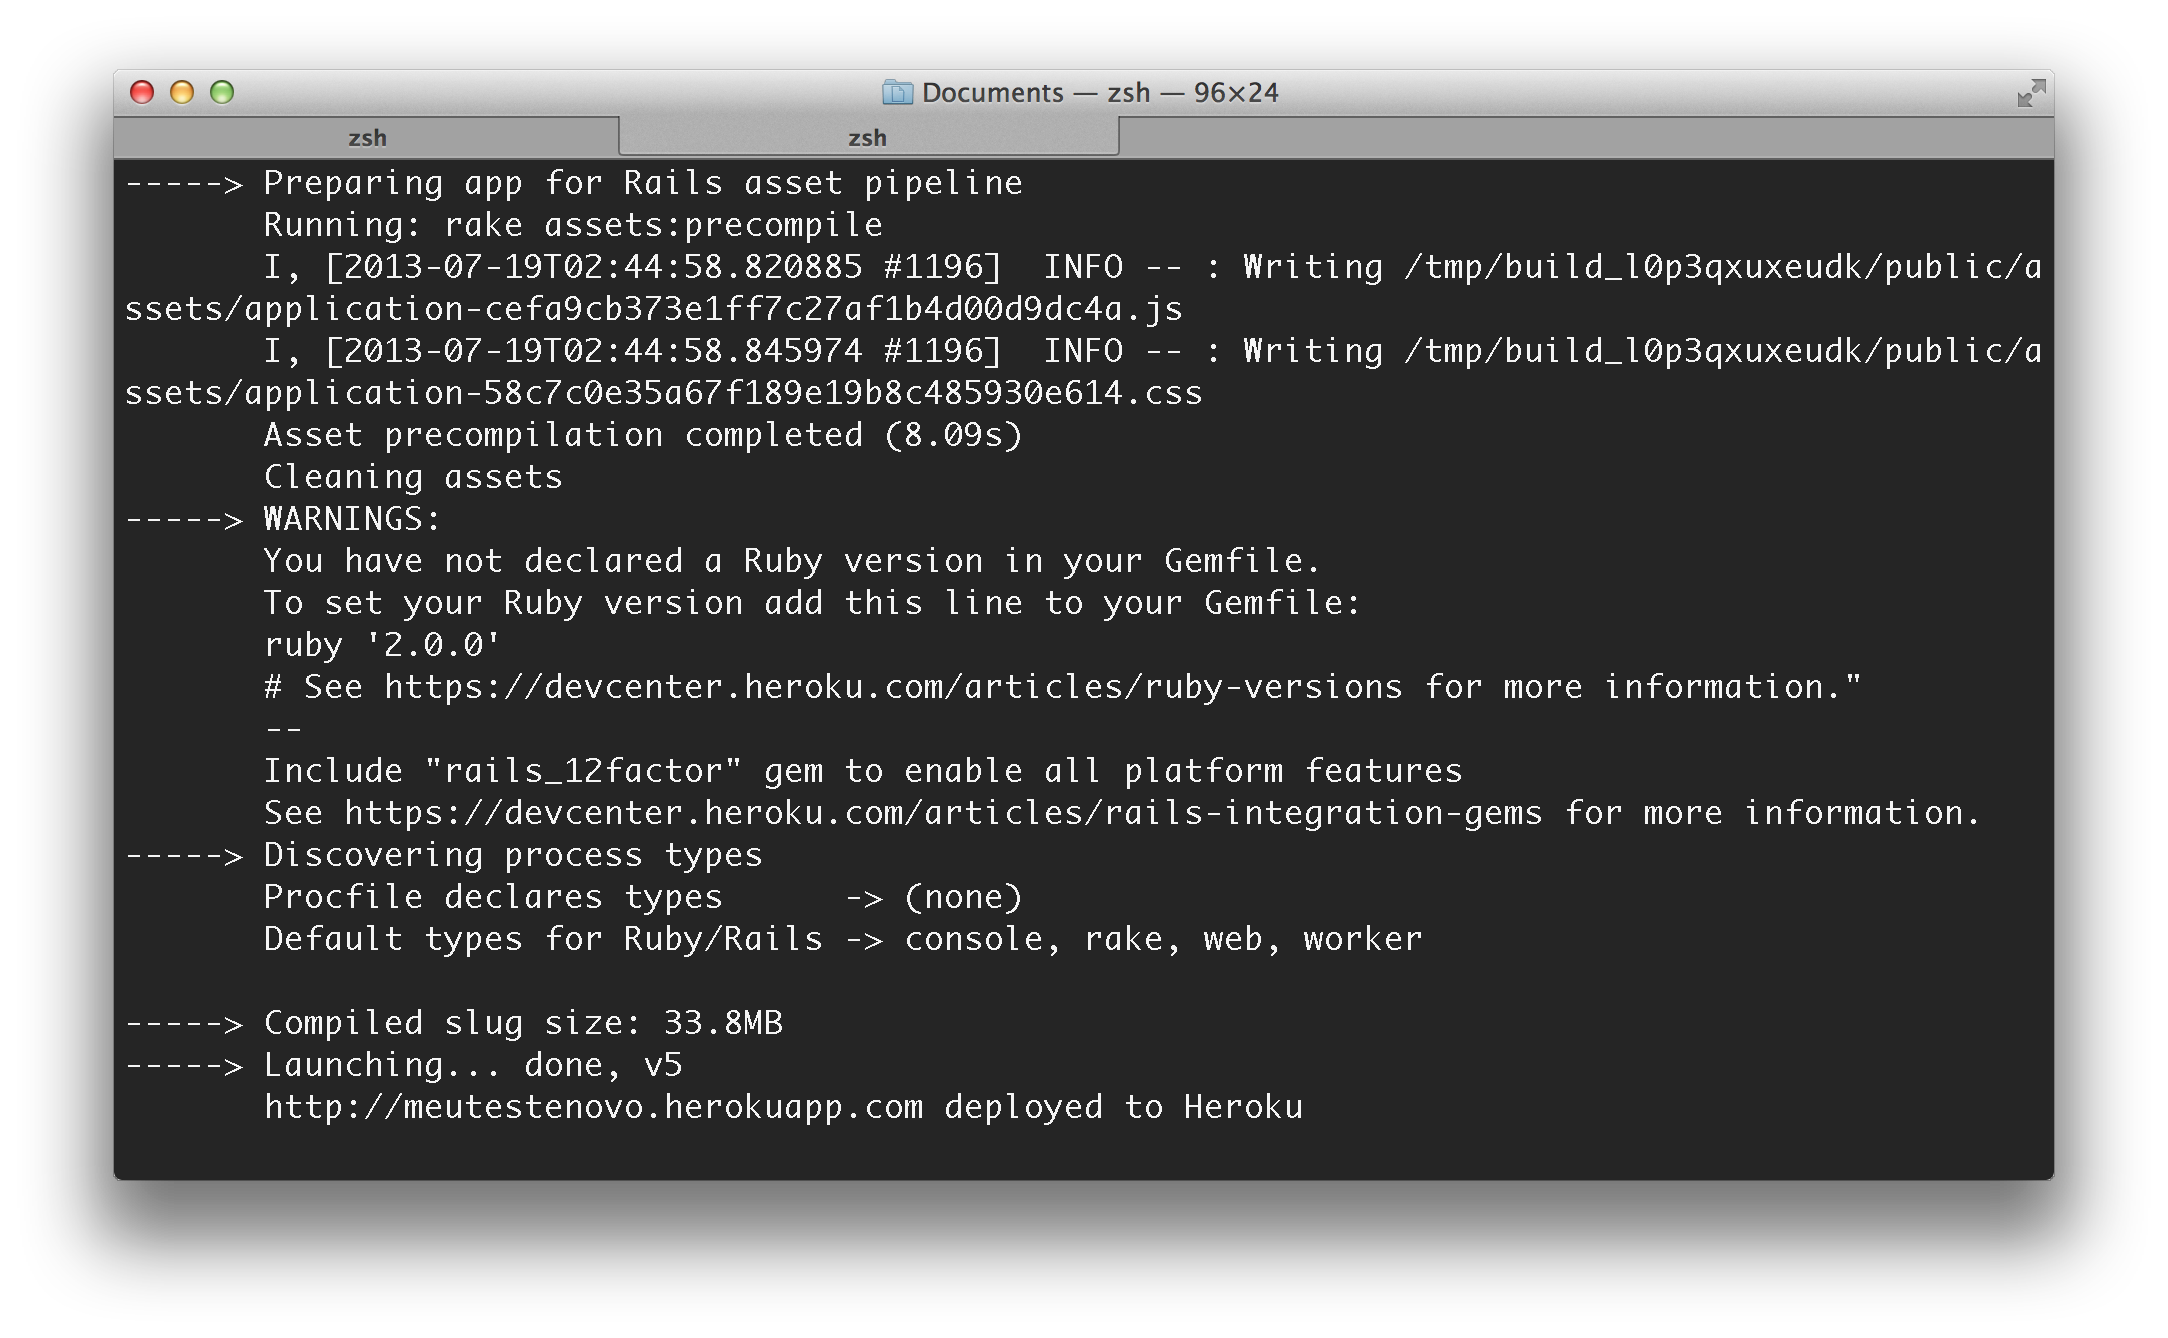
\includegraphics[width=0.5\textwidth]{./fig/setup5}
  \label{fig:fig13}
\end{figure}


